%%%%%%%%%%%%%%%%%%%%%%%%%%%%%%%%%%%%%%%%%
%
% This document will generate an invitation.
% It is intended to be called from a Java program
% which processes a member registry, extracts the
% relevant data to the file personalinfo.tex and
% then compiles this document.
%
% == Compiling LaTeX ==
% xelatex invite.tex
%
%
% == LaTeX prerequisites ==
% sudo apt-get install texlive-full texlive-xetex texlive-lang-european
%
% Extract the zip file from src/main/resources/pgfornament.zip
% The zip originates from: http://altermundus.com/pages/tkz/ornament/index.html
% cd pgfornament
% mkdir -p ~/texmf/tex/latex/
% mkdir -p ~/texmf/tex/generic/
%
% cp pgflibraryam.code.tex pgflibraryvectorian.code.tex pgfornament.sty ~/texmf/tex/latex/
% cp -r am vectorian ~/texmf/tex/generic/
%
%%%%%%%%%%%%%%%%%%%%%%%%%%%%%%%%%%%%%%%%%

\PassOptionsToPackage{svgnames}{xcolor}
\documentclass[a4paper, oneside, final]{scrartcl} % Paper options using the scrartcl class

\usepackage[swedish]{babel}
\usepackage{fontspec} % Allows font customization
\usepackage[bottom=1cm,top=2cm]{geometry}
\usepackage{ifthen}
\usepackage{varwidth}
\usepackage[object=vectorian]{pgfornament} %%  http://altermundus.com/pages/tkz/ornament/index.html

\usetikzlibrary{shapes.geometric,calc}


\include{personalinfo}

\newcommand{\membertypeUngdom}{Ungdom}
\newcommand{\membertypeEnskildmedlem}{Enskild medlem}
\newcommand{\membertypeStudent}{Student}
\newcommand{\membertypeFamilj}{Familj}
\newcommand{\membertypeJuridiskperson}{Juridisk person}
\newcommand{\membertypeHedersmedlem}{Hedersmedlem}

\newcommand{\priceUngdom}{95}
\newcommand{\priceEnskildmedlem}{295}
\newcommand{\priceStudent}{\priceEnskildmedlem{}}
\newcommand{\priceFamilj}{395}
\newcommand{\priceJuridiskperson}{500}
\newcommand{\priceHedermedlem}{0}

% Remove the category "Student"
\newcommand{\membertypeLower}{\ifthenelse{\equal{\membertype}{\membertypeStudent}}{\MakeLowercase{\membertypeEnskildmedlem{}}}{\MakeLowercase{\membertype{}}}}

% Set the correct price based on the member type
\newcommand{\membertypeprice}{\ifthenelse{\equal{\membertype}{\membertypeUngdom}}{\priceUngdom}{\ifthenelse{\equal{\membertype}{\membertypeEnskildmedlem}}{\priceEnskildmedlem}{\ifthenelse{\equal{\membertype}{\membertypeStudent}}{\priceStudent}{\ifthenelse{\equal{\membertype}{\membertypeFamilj}}{\priceFamilj}{\ifthenelse{\equal{\membertype}{\membertypeJuridiskperson}}{\priceJuridiskperson}{\ifthenelse{\equal{\membertype}{\membertypeHedersmedlem}}{\hedersmedlemspris}{}}}}}}}

\newcommand{\swishtext}{Vi tar nu även \textbf{Swish: 1234 018 495}\\}

% Some word constants
\newcommand{\addresstext}{Adress}
\newcommand{\telephonetext}{Telefon}
\newcommand{\mobiletext}{Mobil}
\newcommand{\emailtext}{E-post}
\newcommand{\missingtext}{Saknas}

\newcommand{\currentyear}{2020}
\newcommand{\plats}{Söndag \currentyear{}-02-23 klockan 12:00}
\newcommand{\motionsdeadline}{14/2}

\newcommand{\personalpronounackdat}{\ifthenelse{\equal{\membertype}{\membertypeFamilj}}{er}{dig}}
\newcommand{\personalpronounnominativ}{\ifthenelse{\equal{\membertype}{\membertypeFamilj}}{ni}{du}}
\newcommand{\personalpronounneutrum}{\ifthenelse{\equal{\membertype}{\membertypeFamilj}}{ert}{ditt}}

% Set the title if it is a family
\newcommand{\familytitle}{\ifthenelse{\equal{\membertype}{\membertypeFamilj}}{Familjen}{}}
\newcommand{\membername}{\ifthenelse{\equal{\membertype}{\membertypeFamilj}}{\familytitle{} \membersurnames{} (\memberfirstNames)}{\memberfirstNames{} \membersurnames{}}}


\newcommand{\paymenttext}{
  Glöm inte att betala in medlemsavgiften!\\För att förnya \personalpronounneutrum{} medlemskap som \membertypeLower{}, vänligen betala in \textbf{\membertypeprice{} kr}.\\\swishtext{}\textbf{Plusgiro: 68 03 83 - 7}\\Ange namn på inbetalningen!\\[0.3\baselineskip]
  \membertypeUngdom{} (tom 19 år): \priceUngdom{} kr ~$\cdot{}$~ \membertypeFamilj{}: \priceFamilj{} kr\\
  \membertypeEnskildmedlem{}: \priceEnskildmedlem{} kr\\
}

\newcommand{\memberdetailstext}{Slutligen så ber vi \personalpronounackdat{} hjälpa oss att hålla vårt medlemsregister riktigt. Vänligen mejla \texttt{kontakt@apabepa.cepa} om något av följande inte stämmer:}






%% A macro with two arguments to change ornaments and colors easily
%% Syntax -- \sectionlinetwo{<color>}{<ornament>}
\newcommand{\sectionlinetwo}[2]{%
  \nointerlineskip \vspace{.5\baselineskip}\hspace{\fill}
  {\color{#1}
    \resizebox{0.5\linewidth}{2ex}
    {{%
    {\begin{tikzpicture}
    \node (C) at (0,0) {};
    \node (D) at (9,0) {};
    \path (C) to [ornament=#2] (D);
    \end{tikzpicture}}}}}%
    \hspace{\fill}
    \par\nointerlineskip \vspace{.5\baselineskip}
  }

%----------------------------------------------------------------------------------------
%   TITLE PAGE
%----------------------------------------------------------------------------------------

\begin{document}
\pagestyle{empty} % Removes page numbers


\centering

\rule{\textwidth}{1.6pt}\vspace*{-\baselineskip}\vspace*{2pt} % Thick horizontal line
\rule{\textwidth}{0.4pt}\\[\baselineskip] % Thin horizontal line

{\Huge ÅRSMÖTE \\[0.4\baselineskip]\Large Sällskapet Vikingatida Skepp}\\[0.2\baselineskip] % Title

\rule{\textwidth}{0.4pt}\vspace*{-\baselineskip}\vspace{3.2pt} % Thin horizontal line
\rule{\textwidth}{1.6pt}\\[\baselineskip] % Thick horizontal line

{\scshape % Small caps
\plats{} \\[\baselineskip]
Klubb Maritim, Kajutan\\[0.2\baselineskip]
Sockerbruket 17\\[0.2\baselineskip]
Göteborg\par}

\vspace*{\baselineskip}
\sectionlinetwo{black}{89}
\vspace*{\baselineskip}

\begin{varwidth}{\textwidth}
\begin{itemize}
\item Årsmötesförhandlingar
\item Motion: Försäljning/avyttring av Starkodder
\item Val av styrelse
\item Arbetsdagar \currentyear{}
\end{itemize}
\end{varwidth}

\vspace*{1.5\baselineskip}
Preliminära mötesdokument finns på \texttt{vidfamne.se/arsmote-2020}\\[0.8\baselineskip]

Motioner ska vara inne senast \motionsdeadline{}, adress: \texttt{kontakt@apabepa.cepa}\\
Soppa (vegetarisk vid förfrågan), kaffe och liten kaka serveras.\\[0.8\baselineskip]

För att kunna planera maten vill vi gärna att \personalpronounnominativ{} anmäler \personalpronounackdat{}. Skriv till \texttt{kontakt@apabepa.cepa} eller ring ordförande Johan på 0700-12 34 56.

\vspace*{\baselineskip}

\ifthenelse{\not\equal{\membertype}{\membertypeHedersmedlem}}{
  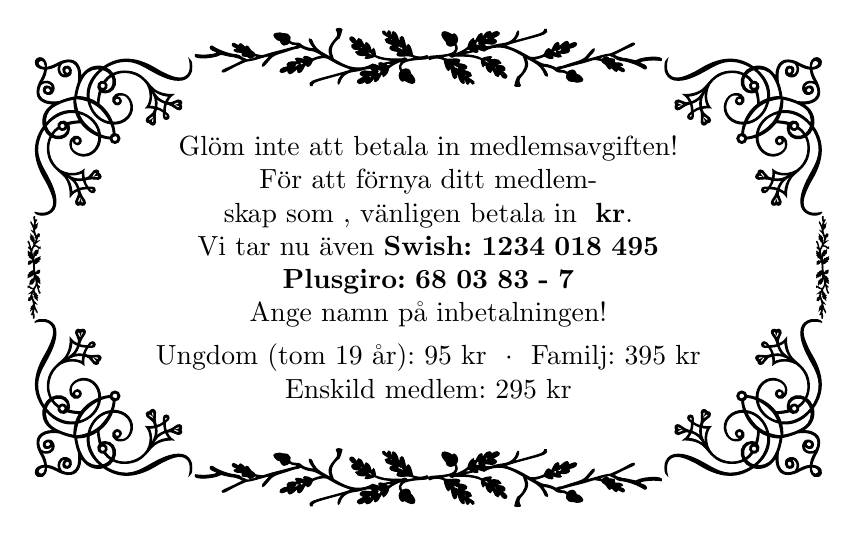
\begin{tikzpicture}[every node/.style={inner sep=0pt}]
  \node[text width=8cm,align=center](Text){%
    \paymenttext{}
  } ;
  \node[shift={(-1cm,1cm)},anchor=north west](CNW)  at (Text.north west)
                 {\pgfornament[width=2cm]{61}};
  \node[shift={(1cm,1cm)},anchor=north east](CNE)   at (Text.north east)
                 {\pgfornament[width=2cm,symmetry=v]{61}};
  \node[shift={(-1cm,-1cm)},anchor=south west](CSW) at (Text.south west)
                 {\pgfornament[width=2cm,symmetry=h]{61}};
  \node[shift={(1cm,-1cm)},anchor=south east](CSE)  at (Text.south east)
                 {\pgfornament[width=2cm,symmetry=c]{61}};
  \pgfornamenthline{CNW}{CNE}{north}{87}
  \pgfornamenthline{CSW}{CSE}{south}{87}
  \pgfornamentvline{CNW}{CSW}{west}{87}
  \pgfornamentvline{CNE}{CSE}{east}{87}
  \end{tikzpicture}
}{
  \sectionlinetwo{black}{89}
}

\vspace*{\baselineskip}

\memberdetailstext{}\\[0.7\baselineskip]
{\scshape % Small caps
\membername{}\\
\ifthenelse{\equal{\memberaddress}{}}{\addresstext{}: \textbf{\missingtext{}}}{\memberstreet{}, \memberaddress{}}\\
\ifthenelse{\equal{\membertelephone}{}}{\ifthenelse{\equal{\membermobile}{}}{\telephonetext{}: \textbf{\missingtext{}}\\}{}}{}
\ifthenelse{\equal{\membertelephone}{}}{}{\telephonetext{}: \membertelephone{}\\}
\ifthenelse{\equal{\membermobile}{}}{}{\mobiletext{}: \membermobile{}\\}
\emailtext{}: \ifthenelse{\equal{\memberemail}{}}{\textbf{\missingtext{}}}{\memberemail{}}\\
}

\end{document}
